%		\def\sphinxdocclass{report}
%\documentclass[letterpaper,10pt,spanish]{sphinxmanual}
%\ifdefined\pdfpxdimen
%   \let\sphinxpxdimen\pdfpxdimen\else\newdimen\sphinxpxdimen
%\fi \sphinxpxdimen=.75bp\relax
%
%\PassOptionsToPackage{warn}{textcomp}
%\usepackage[utf8]{inputenc}
%\ifdefined\DeclareUnicodeCharacter
% \ifdefined\DeclareUnicodeCharacterAsOptional
%  \DeclareUnicodeCharacter{"00A0}{\nobreakspace}
%  \DeclareUnicodeCharacter{"2500}{\sphinxunichar{2500}}
%  \DeclareUnicodeCharacter{"2502}{\sphinxunichar{2502}}
%  \DeclareUnicodeCharacter{"2514}{\sphinxunichar{2514}}
%  \DeclareUnicodeCharacter{"251C}{\sphinxunichar{251C}}
%  \DeclareUnicodeCharacter{"2572}{\textbackslash}
% \else
%  \DeclareUnicodeCharacter{00A0}{\nobreakspace}
%  \DeclareUnicodeCharacter{2500}{\sphinxunichar{2500}}
%  \DeclareUnicodeCharacter{2502}{\sphinxunichar{2502}}
%  \DeclareUnicodeCharacter{2514}{\sphinxunichar{2514}}
%  \DeclareUnicodeCharacter{251C}{\sphinxunichar{251C}}
%  \DeclareUnicodeCharacter{2572}{\textbackslash}
% \fi
%\fi
%\usepackage{cmap}
%\usepackage[T1]{fontenc}
%\usepackage{amsmath,amssymb,amstext}
%\usepackage{babel}
%\usepackage[Sonny]{fncychap}
%\usepackage{sphinx}
%
%\usepackage{breakurl}
%\usepackage{geometry}
%
%% Include hyperref last.
%\usepackage{hyperref}
%% Fix anchor placement for figures with captions.
%\usepackage{hypcap}% it must be loaded after hyperref.
%% Set up styles of URL: it should be placed after hyperref.
%\urlstyle{same}
%\addto\captionsspanish{\renewcommand{\contentsname}{Contents:}}
%
%\addto\captionsspanish{\renewcommand{\figurename}{Figura}}
%\addto\captionsspanish{\renewcommand{\tablename}{Tabla}}
%\addto\captionsspanish{\renewcommand{\literalblockname}{Lista}}
%
%\addto\captionsspanish{\renewcommand{\literalblockcontinuedname}{proviene de la página anterior}}
%\addto\captionsspanish{\renewcommand{\literalblockcontinuesname}{continues on next page}}
%
%\addto\extrasspanish{\def\pageautorefname{página}}
%

%\begin{document}

\section{Implementación del servicio sobre CloudNAO}



Para crear y probar cada una de las arquitecturas que se
describieron en la sección anterior se utilizó la biblioteca
de TensorFlow.
Se construyó una clase que pudiera crear gráficas de modelos
con los cuatro casos antes descritos y luego se automatizó el proceso de
entrenamiento de todas las posibles arquitecturas, variando los parámetros.
Así, cada instancia de la clase, es un modelo diferente. En esta sección se 
describe la implementación de las CNN, su entrenamiento, evaluación
y lanzamiento sobre la API REST de CloudNAO.


El programa en TensorFlow encargado del entrenamiento de la CNN se puede dividir en tres partes principales; la primera es la carga las imágenes de cada conjunto a partir de su ruta y su etiquetado, en la segunda
se crean las gráficas de cómputo y por último se ejecutan esas gráficas de cómputo.

Para agregar el modelo a la API de CloudNAO sólo se añadió un nuevo módulo
al recurso \texttt{/vision}, en donde se carga la gráfica de cómputo 
con los mejores resultados.

%%%%%%%%%%%%%%%%%%%%%%%%%%%%%%%%%%%%%%%%%%%%%%%%%%%%%%%%%%%%%%%%
%%%%%%%%%%%%%%%%%%%%%%%%%%%%%%%%%%%%%%%%%%%%%%%%%%%%%%%%%%%%%%%%
%%%%%%%%%%%%%%%%%%%%%%%%%%%%%%%%%%%%%%%%%%%%%%%%%%%%%%%%%%%%%%%%


\subsection{Hardware y software}

El hardware sobre el que se realizó el entrenamiento de las
diferentes arquitecturas fue un equipo con las siguientes características:

\begin{itemize}

\item Procesador: Intel Core i5-7300HQ CPU 2.50GHz x 4.
\item Memoria RAM: 8GB.
\item GPU:  NVIDIA GeForce GTX 1050 2GB.
\item SSD: 250 GB.
\end{itemize}

Como ya se explicó, la biblioteca para desarrollar el modelo en Python fue TensorFlow, la cual cuenta
con soporte para la plataforma de cómputo paralelo CUDA (Arquitectura
Unificada de Dispositivos de Cómputo), desarrollada por NVIDIA.
La versión de CUDA y de TensorFlow (con soporte para GPU) fueron 8.0 y 1.4.0, respectivamente.

Además de TensorFlow, las otras dos bibliotecas importantes son 
\texttt{numpy} y \texttt{opencv}, principalmente para la carga de
las imágenes en un formato que pudiera recibir la CNN.


%%%%%%%%%%%%%%%%%%%%%%%%%%%%%%%%%%%%%%%%%%%%%%%%%%%%%%%%%%%%%%%%%%%%%%%%%%%%%%%%%%%%%%%%%%%%%%%%%%%%%%%%%%%%%%%%%%%%%%%%%%%%%%%%%%%%%%%%%%%%%%%%%%%%%%%%%%%%%%%%%%%%%%%%%%%%%%%%%%%%%%%%%%%%%%%%%%%%%%%%%%%%%%%%%
\subsection{Preparación del conjunto de datos}

Contamos con un conjunto de entrenamiento de $6000$ imágenes y 
un conjunto de prueba de $2112$.
Como estamos utilizando un algoritmo de aprendizaje supervisado, 
se necesitan etiquetas u objetivos para cada imagen. La representación
de esas etiquetas se hizo con vectores $\mathbf{y}$ en codificación one-hot,
con $y_n = 1$ si la imagen pertenece a la clase $n$ y $y_i = 0$ para todos los
demás casos. Los vectores posibles de acuerdo las cuatro categorías son los siguientes:

\begin{itemize}
\item $(1, 0, 0, 0)$ si la imagen es de la categoría \textit{zona de trabajo}.
\item $(0, 1, 0, 0)$ si la imagen es de la categoría \textit{salida}.
\item $(0, 0, 1, 0)$ si la imagen es de la categoría \textit{cubículo}.
\item $(0, 0, 0, 1)$ si la imagen es de la categoría \textit{cancha}.
\end{itemize}

Esta codificación se puede interpretar como una distribución de probabilidad
sobre las cuatro clases.

Se definió un módulo \texttt{cnn\_indoor\_classifier\_model} con 
una clase \texttt{CNNClassifier\\LAR}
que encapsula los métodos para la carga de las imágenes, su 
procesamiento, la definición de la gráfica de cómputo y la ejecución.
Dentro de la clase el método \texttt{get\_training\_and\_test\_images()}
carga y procesa las imágenes para definir los conjuntos de entrenamiento
y de prueba para nuestro modelo.
Primero se obtiene la ruta de cada imagen y se crea la lista con las etiquetas
(vectores one-hot)
de cada imagen dependiendo de la carpeta donde se encontraba, luego con
\sphinxcode{\sphinxupquote{opencv}} se cargan las imágenes a la memoria como arreglos de
\sphinxcode{\sphinxupquote{numpy}}, se redimensionan a un tamaño de $32 \times 32$ y se normalizan
los valores de los pixeles. Al final se tienen dos arreglos de \sphinxcode{\sphinxupquote{numpy}}
donde cada elemento es un arreglo de tres dimensiones que
representa una imagen. El código de las operaciones dentro del método
son las siguientes:

\fvset{hllines={, ,}}%
\begin{sphinxVerbatim}[commandchars=\\\{\}]
\PYG{c+c1}{\PYGZsh{} Carga del conjunto de entrenamiento}
\PYG{n}{training\PYGZus{}paths} \PYG{o}{=} \PYG{n}{np}\PYG{o}{.}\PYG{n}{array}\PYG{p}{(}\PYG{n}{list\PYGZus{}files\PYGZus{}in\PYGZus{}directory}\PYG{p}{(}\PYG{l+s+s1}{\PYGZsq{}}\PYG{l+s+s1}{dataset/training\PYGZus{}set/*}\PYG{l+s+s1}{\PYGZsq{}}\PYG{p}{)}\PYG{p}{)}
\PYG{n}{np}\PYG{o}{.}\PYG{n}{random}\PYG{o}{.}\PYG{n}{shuffle}\PYG{p}{(}\PYG{n}{training\PYGZus{}paths}\PYG{p}{)}
\PYG{n}{labels\PYGZus{}training\PYGZus{}set} \PYG{o}{=} \PYG{n}{get\PYGZus{}labels\PYGZus{}from\PYGZus{}path}\PYG{p}{(}\PYG{n}{training\PYGZus{}paths}\PYG{p}{)}
\PYG{n}{training\PYGZus{}images} \PYG{o}{=} \PYG{n}{np}\PYG{o}{.}\PYG{n}{array}\PYG{p}{(}\PYG{p}{[}\PYG{n}{cv2}\PYG{o}{.}\PYG{n}{cvtColor}\PYG{p}{(}\PYG{n}{cv2}\PYG{o}{.}\PYG{n}{resize}\PYG{p}{(}\PYG{n}{cv2}\PYG{o}{.}\PYG{n}{imread}\PYG{p}{(}\PYG{n}{file\PYGZus{}name}\PYG{p}{)}\PYG{p}{,} \PYG{p}{(}\PYG{l+m+mi}{32}\PYG{p}{,} \PYG{l+m+mi}{32}\PYG{p}{)}\PYG{p}{)}\PYG{p}{,} \PYG{n}{cv2}\PYG{o}{.}\PYG{n}{COLOR\PYGZus{}BGR2RGB}\PYG{p}{)} \PYG{o}{/} \PYG{l+m+mi}{255} \PYG{k}{for} \PYG{n}{file\PYGZus{}name} \PYG{o+ow}{in} \PYG{n}{training\PYGZus{}paths}\PYG{p}{]}\PYG{p}{)}
\PYG{c+c1}{\PYGZsh{} Conjunto de prueba}
\PYG{n}{testing\PYGZus{}paths} \PYG{o}{=} \PYG{n}{np}\PYG{o}{.}\PYG{n}{array}\PYG{p}{(}\PYG{n}{list\PYGZus{}files\PYGZus{}in\PYGZus{}directory}\PYG{p}{(}\PYG{l+s+s1}{\PYGZsq{}}\PYG{l+s+s1}{dataset/test\PYGZus{}set/*}\PYG{l+s+s1}{\PYGZsq{}}\PYG{p}{)}\PYG{p}{)}
\PYG{n}{np}\PYG{o}{.}\PYG{n}{random}\PYG{o}{.}\PYG{n}{shuffle}\PYG{p}{(}\PYG{n}{testing\PYGZus{}paths}\PYG{p}{)}
\PYG{n}{labels\PYGZus{}test\PYGZus{}set} \PYG{o}{=} \PYG{n}{get\PYGZus{}labels\PYGZus{}from\PYGZus{}path}\PYG{p}{(}\PYG{n}{testing\PYGZus{}paths}\PYG{p}{)}
\PYG{n}{testing\PYGZus{}images} \PYG{o}{=} \PYG{n}{np}\PYG{o}{.}\PYG{n}{array}\PYG{p}{(}\PYG{p}{[}\PYG{n}{cv2}\PYG{o}{.}\PYG{n}{cvtColor}\PYG{p}{(}\PYG{n}{cv2}\PYG{o}{.}\PYG{n}{resize}\PYG{p}{(}\PYG{n}{cv2}\PYG{o}{.}\PYG{n}{imread}\PYG{p}{(}\PYG{n}{file\PYGZus{}name}\PYG{p}{)}\PYG{p}{,} \PYG{p}{(}\PYG{l+m+mi}{32}\PYG{p}{,} \PYG{l+m+mi}{32}\PYG{p}{)}\PYG{p}{)}\PYG{p}{,} \PYG{n}{cv2}\PYG{o}{.}\PYG{n}{COLOR\PYGZus{}BGR2RGB}\PYG{p}{)} \PYG{o}{/}\PYG{l+m+mi}{255} \PYG{k}{for} \PYG{n}{file\PYGZus{}name} \PYG{o+ow}{in} \PYG{n}{testing\PYGZus{}paths}\PYG{p}{]}\PYG{p}{)}
\end{sphinxVerbatim}



%%%%%%%%%%%%%%%%%%%%%%%%%%%%%%%%%%%%%%%%%%%%%%%%%%%%%%%%%%%%%%%%%%%%%%
%%%%%%%%%%%%%%%%%%%%%%%%%%%%%%%%%%%%%%%%%%%%%%%%%%%%%%%%%%%%%%%%%%%%%%
%%%%%%%%%%%%%%%%%%%%%%%%%%%%%%%%%%%%%%%%%%%%%%%%%%%%%%%%%%%%%%%%%%%%

\subsection{Construcción del modelo en TensorFlow}
\label{\detokenize{model_desc:creacion-y-ejecucion-de-la-grafica-de-tensorflow}}

\subsubsection{Definición del modelo}

Para la implementación de la CNN en TensorFlow
se utilizó una clase que representara una
arquitectura. Esto fue para que experimentar con
una estructura y parámetros diferentes sólo
implicara instanciar un objeto de la clase.
La clase se llama \sphinxcode{\sphinxupquote{CNNClassifierLAR}} y
está dentro del módulo {\hyperref[\detokenize{model_desc:module-cnn\_indoor\_classifier\_model}]{\sphinxcrossref{\sphinxcode{\sphinxupquote{cnn\_indoor\_classifier\_model}}}}}.
El módulo anterior además de la clase contiene múltiples
funciones auxiliares para facilitar la definición
de los parámetros de aprendizaje, la operaciones entre los
tensores, la obtención de las rutas de las imágenes
y la generación de los vectores one-hot de sus etiquetas.

Se pueden construir hasta cuatro tipos distintos de
arquitecturas, con dos capas convolucionales con una o dos
completamente conectadas, y con una capa de convolución
y uno o dos completamente conectadas.
La construcción de éstas se hace con los métodos
\texttt{create\_graph\_2\_convo\_layers()}
y \texttt{create\_graph\_1\_convo\_layer()}
que reciben como argumento una bandera para construir su gráfica
de cómputo con dos o una capa completamente conectada. A
continuación se desglosan los pasos del método para
crear la gráfica con dos capas de convolución.

\begin{enumerate}

\item La creación de la primera de convolución, recibe como entradas el placeholder
con las imágenes y a la función se le pasan como parámetros una lista con las dimensiones
de los kernels que se aplican y el número de mapas de características. Por ejemplo
un lista \sphinxcode{\sphinxupquote{{[}5, 5, 3, 16{]}}} indica que se deben aplicar kernels de $5 \times 5$ a
una entrada con 3 canales (la imagen RGB), para obtener
16 mapas de características, después se aplica un agrupamiento para disminuir las
dimensiones de los 16 mapas a la mitad:

\fvset{hllines={, ,}}%
\begin{sphinxVerbatim}[commandchars=\\\{\}]
\PYG{n}{convo\PYGZus{}1} \PYG{o}{=} \PYG{n}{convolutional\PYGZus{}layer}\PYG{p}{(}\PYG{n}{input\PYGZus{}x\PYGZus{}ph}\PYG{p}{,} \PYG{n}{shape}\PYG{p}{)}
\PYG{n}{convo\PYGZus{}1\PYGZus{}pooling} \PYG{o}{=} \PYG{n}{max\PYGZus{}pool\PYGZus{}2by2}\PYG{p}{(}\PYG{n}{convo\PYGZus{}1}\PYG{p}{)}
\end{sphinxVerbatim}

\item Luego sigue la otra capa de convolución que tiene como entrada las salidas
de la capa anterior. Se aplica de nuevo un agrupamiento para reducir las al $50\%$ las
dimensiones de la imagen:

\fvset{hllines={, ,}}%
\begin{sphinxVerbatim}[commandchars=\\\{\}]
\PYG{n}{convo\PYGZus{}2} \PYG{o}{=} \PYG{n}{convolutional\PYGZus{}layer}\PYG{p}{(}\PYG{n}{convo\PYGZus{}1\PYGZus{}pooling}\PYG{p}{,} \PYG{n}{shape}\PYG{p}{)}
\PYG{n}{convo\PYGZus{}2\PYGZus{}pooling} \PYG{o}{=} \PYG{n}{max\PYGZus{}pool\PYGZus{}2by2}\PYG{p}{(}\PYG{n}{convo\PYGZus{}2}\PYG{p}{)}
\end{sphinxVerbatim}

\item Se redimensionan los
mapas de características para tener una red neuronal donde cada unidad es un
elemento dentro del mapa de características. Esto es equivalente a aplicar
una convolución con kernel de $1 \times 1$. 
Se conectan las unidades de la capa a una nueva capa oculta
completamente conectada.

\fvset{hllines={, ,}}%
\begin{sphinxVerbatim}[commandchars=\\\{\}]
\PYG{n}{convo\PYGZus{}2\PYGZus{}flat} \PYG{o}{=} \PYG{n}{tf}\PYG{o}{.}\PYG{n}{reshape}\PYG{p}{(}\PYG{n}{convo\PYGZus{}2\PYGZus{}pooling}\PYG{p}{,} \PYG{p}{[}\PYG{o}{\PYGZhy{}}\PYG{l+m+mi}{1}\PYG{p}{,} \PYG{l+m+mi}{8} \PYG{o}{*} \PYG{l+m+mi}{8} \PYG{o}{*} \PYG{n}{last\PYGZus{}maps\PYGZus{}of\PYGZus{}features}\PYG{p}{]}\PYG{p}{)}
\PYG{n}{full\PYGZus{}layer\PYGZus{}one} \PYG{o}{=} \PYG{n}{tf}\PYG{o}{.}\PYG{n}{nn}\PYG{o}{.}\PYG{n}{relu}\PYG{p}{(}\PYG{n}{normal\PYGZus{}full\PYGZus{}layer}\PYG{p}{(}\PYG{n}{convo\PYGZus{}2\PYGZus{}flat}\PYG{p}{,} \PYG{n}{units\PYGZus{}fc}\PYG{p}{)}\PYG{p}{)}
\end{sphinxVerbatim}

\item La última capa es el vector predicho, que se pasa por la función softmax para
medir el error con la entropía cruzada. Finalmente se tiene la operación
\sphinxcode{\sphinxupquote{train}} que minimiza la función de costo utilizando el algoritmo de
retropropagación:

\fvset{hllines={, ,}}%
\begin{sphinxVerbatim}[commandchars=\\\{\}]
\PYG{n}{y\PYGZus{}pred} \PYG{o}{=} \PYG{n}{tf}\PYG{o}{.}\PYG{n}{identity}\PYG{p}{(}\PYG{n}{normal\PYGZus{}full\PYGZus{}layer}\PYG{p}{(}\PYG{n}{full\PYGZus{}layer\PYGZus{}one}\PYG{p}{,} \PYG{l+m+mi}{4}\PYG{p}{)}\PYG{p}{)}
\PYG{n}{cross\PYGZus{}entropy} \PYG{o}{=} \PYG{n}{tf}\PYG{o}{.}\PYG{n}{reduce\PYGZus{}mean}\PYG{p}{(}\PYG{n}{tf}\PYG{o}{.}\PYG{n}{nn}\PYG{o}{.}\PYG{n}{softmax\PYGZus{}cross\PYGZus{}entropy\PYGZus{}with\PYGZus{}logits}\PYG{p}{(}\PYG{n}{labels}\PYG{o}{=}\PYG{n}{y\PYGZus{}true\PYGZus{}ph}\PYG{p}{,} \PYG{n}{logits}\PYG{o}{=}\PYG{n}{y\PYGZus{}pred}\PYG{p}{)}\PYG{p}{)}
\PYG{n}{optimizer} \PYG{o}{=} \PYG{n}{tf}\PYG{o}{.}\PYG{n}{train}\PYG{o}{.}\PYG{n}{GradientDescentOptimizer}\PYG{p}{(}\PYG{n}{learning\PYGZus{}rate}\PYG{o}{=}\PYG{n}{learning\PYGZus{}rate}\PYG{p}{)}
\PYG{n}{train} \PYG{o}{=} \PYG{n}{optimizer}\PYG{o}{.}\PYG{n}{minimize}\PYG{p}{(}\PYG{n}{loss}\PYG{o}{=}\PYG{n}{cross\PYGZus{}entropy}\PYG{p}{,} \PYG{n}{global\PYGZus{}step}\PYG{o}{=}\PYG{n}{tf}\PYG{o}{.}\PYG{n}{train}\PYG{o}{.}\PYG{n}{get\PYGZus{}global\PYGZus{}step}\PYG{p}{(}\PYG{p}{)}\PYG{p}{)}
\end{sphinxVerbatim}


\end{enumerate}


\subsubsection{Ejecución}

La ejecución de la gráfica de cómputo de una instancia
es con el método \texttt{run\_graph()}.
Se pasan como parámetro el número de épocas y el tamaño del lote
para el aprendizaje.
Este método ejecuta la operación
\sphinxcode{\sphinxupquote{train}} que a su vez corre todas las operaciones que la preceden.
Cada 100 épocas se evalúa la precisión del modelo y se imprimen:
el número de época, el tiempo transcurrido desde que se inició el entrenamiento, el error de entrenamiento, el error de prueba y
la precisión.


\codedocumentation{\sphinxbfcode{\sphinxupquote{class }}\sphinxcode{\sphinxupquote{cnn\_indoor\_classifier\_model.}}\sphinxbfcode{\sphinxupquote{CNNClassifierLAR}}{(\emph{shape\_convo\_layers}, \emph{units\_fc}, \emph{learning\_rate}})}

La clase que representa una arquitectura de red convolucional con a lo más
dos capas de convolución y dos capas completamente conectadas.

La red está creada para específicamente aceptar entradas de dimensiones
de 32 pixeles por 32 pixeles por 3 canales. El constructor recibe tres parámetros
una lista con las dimensiones de los kernels, entradas de la convolución y
número de mapas de características, un entero con el número de unidades en la
capa oculta y un valor flotante que es la tasa de aprendizaje.
En el siguiente ejemplo se crea una red con dos capas de convolución,
una capa oculta con 2048 unidades y una tasa de aprendizaje de 0.01. La ejecución de la gráfica
para el aprendizaje por lotes recibe como parámetros 200 y 3000,
el tamaño del lote y el número de épocas, respectivamente.

\fvset{hllines={, ,}}%
\begin{sphinxVerbatim}[commandchars=\\\{\}]
\PYG{g+gp}{\PYGZgt{}\PYGZgt{}\PYGZgt{} }\PYG{k+kn}{from} \PYG{n+nn}{cnn\PYGZus{}indoor\PYGZus{}classifier\PYGZus{}model} \PYG{k}{import} \PYG{n}{CNNClassifierLAR}
\PYG{g+gp}{\PYGZgt{}\PYGZgt{}\PYGZgt{} }\PYG{n}{clasificador} \PYG{o}{=} \PYG{n}{CNNClassifierLAR}\PYG{p}{(}\PYG{p}{[}\PYG{p}{[}\PYG{l+m+mi}{5}\PYG{p}{,} \PYG{l+m+mi}{5}\PYG{p}{,} \PYG{l+m+mi}{3}\PYG{p}{,} \PYG{l+m+mi}{16}\PYG{p}{]}\PYG{p}{,} \PYG{p}{[}\PYG{l+m+mi}{3}\PYG{p}{,} \PYG{l+m+mi}{3}\PYG{p}{,} \PYG{l+m+mi}{16}\PYG{p}{,} \PYG{l+m+mi}{32}\PYG{p}{]}\PYG{p}{]}\PYG{p}{,} \PYG{l+m+mi}{2048}\PYG{p}{,} \PYG{l+m+mf}{0.01}\PYG{p}{)}
\PYG{g+gp}{\PYGZgt{}\PYGZgt{}\PYGZgt{} }\PYG{n}{clasificador}\PYG{o}{.}\PYG{n}{create\PYGZus{}graph\PYGZus{}2\PYGZus{}convo\PYGZus{}layers}\PYG{p}{(}\PYG{p}{)}
\PYG{g+gp}{\PYGZgt{}\PYGZgt{}\PYGZgt{} }\PYG{n}{clasificador}\PYG{o}{.}\PYG{n}{run\PYGZus{}graph}\PYG{p}{(}\PYG{l+m+mi}{200}\PYG{p}{,} \PYG{l+m+mi}{3000}\PYG{p}{)}
\PYG{g+go}{i; time; training loss; test loss; accuracy}
\PYG{g+go}{0;0.7688136100769043;1.5798137187957764;1.4590167999267578;0.13778409361839294}
\PYG{g+gp}{...}
\PYG{g+go}{3000;68.31876397132874;0.0036288381088525057;0.11022621393203735;0.9692234992980957}
\PYG{g+go}{Time 68.3188087940216}
\end{sphinxVerbatim}

%%%%%%%%%%%%%%%%%%%%%%%%%%%%%%%%%%%%%%%%%%%%%%%%%%%%%%%%%%%%%%%%%%%%%%%%%%%%%%%%%%%%%%%%%%%%%%%%%%%%%%%%%%%%%%%%%%%%%%%%%%%%%%%%%%%%%%%%%%%%%%%%%%%%%%%%%%%%%%%%%%%%%%%%%%%%%%%%%%%%%%%%%%%%%%%%%%%%%



\subsection{Resultados}

Después del entrenamiento de los $756$ modelos posibles,
se eligieron aquellos con la precisión más alta de cada una de las cuatro estructuras mencionadas previamente. Éstos se resumen en la tabla \ref{table:models_results}. Las abreviaciones Convo y FC denotan
a capas convolucionales y completamente conectadas, respectivamente.
$\gamma$ denota la tasa de aprendizaje, y el tiempo es la duración
del entrenamiento en segundos.

\begin{table}[!h]
\centering
\caption{Los modelos con la precisiones más altas en cada tipo de
estructura.\label{table:models_results}}

\begin{tabular}{|l|l|l|l|l|l|l|l|l|}
\hline
Modelo                                                           & Épocas & $\gamma$ & Lote & Kernels                                                              & \begin{tabular}[c]{@{}l@{}}Mapas\\ de\\ caracte-\\ rísticas\end{tabular} & \begin{tabular}[c]{@{}l@{}}Unidades\\ de la\\ capas\\ FC\end{tabular} & Precisión & Tiempo \\ \hline
\begin{tabular}[c]{@{}l@{}}(1) \\2 Convo\\ 2 FC\end{tabular} & 2000   & 0.01     & 200  & \begin{tabular}[c]{@{}l@{}}$5 \times 5$,\\ $3 \times 3$\end{tabular} & 16, 32                                                                   & 1024, 4                                                               & 0.97917   & 168.29 \\ \hline
\begin{tabular}[c]{@{}l@{}}(2)\\2 Convo\\2 FC\end{tabular}        & 2000   & 0.01     & 300  & \begin{tabular}[c]{@{}l@{}}$5 \times 5$,\\ $3 \times 3$\end{tabular} & 16, 32                                                                   & 1024, 4                                                               & 0.97917   & 191.71 \\ \hline
\begin{tabular}[c]{@{}l@{}}(3)\\2 Convo\\ 1 FC\end{tabular}  & 2000   & 0.01     & 300  & \begin{tabular}[c]{@{}l@{}}$7 \times 7$,\\ $5 \times 5$\end{tabular} & 16, 32                                                                   & 4                                                                     & 0.97159   & 79.73  \\ \hline
\begin{tabular}[c]{@{}l@{}}(4)\\1 Convo\\ 2 FC\end{tabular}  & 2000   & 0.01     & 200  & $5 \times 5$                                                         & 16                                                                       & 512, 4                                                                & 0.97775   & 119.13 \\ \hline
\begin{tabular}[c]{@{}l@{}}(5)\\1 Convo\\ 1 FC\end{tabular}  & 2000   & 0.01     & 100  & $5 \times 5$                                                         & 32                                                                       & 4                                                                     & 0.96117   & 45.83  \\ \hline
\end{tabular}

\end{table}

Los modelos con la mayor precisión sobre todos son el modelo (1) y
(2) con una proporción de valores correctamente clasificados de
0.97917. Se puede ver que los parámetros que comparten todas
las arquitecturas son el número de épocas y la tasa de aprendizaje,
además de que en sus kernels aparece al menos uno con una dimensión 
de $5 \times 5$. Los mapas de características producidos 
por las capas de convolución no son menores a $16$, lo que podría
indicar que podríamos añadir más mapas para mejorar el modelo.

La diferencia entre tiempo y la precisión entre los cinco modelos
no es significativa. Todos están por arriba del $0.96$
en cuanto a la precisión. La diferencia del tiempo de entrenamiento 
entre los modelos es mínima, un par de minutos entre el modelo (2) y (5),
lo que no es nada en comparación a modelos más complejos que tardan horas
sobre sistemas con un gran poder de cómputo.


En la figura \ref{fig:results_acc_epochs}
podemos ver que la precisión de cada modelo, a pesar de que 
sí mejora con respecto a las épocas, converge muy rápidamente.
Aproximadamente desde la época $300$,
el incremento de la precisión es lento pero está por arriba
del $0.95$.


\begin{figure}[!ht]
\renewcommand*\thesubfigure{\arabic{subfigure}} 
  \centering
\subfloat[2 Convo 2 FC]{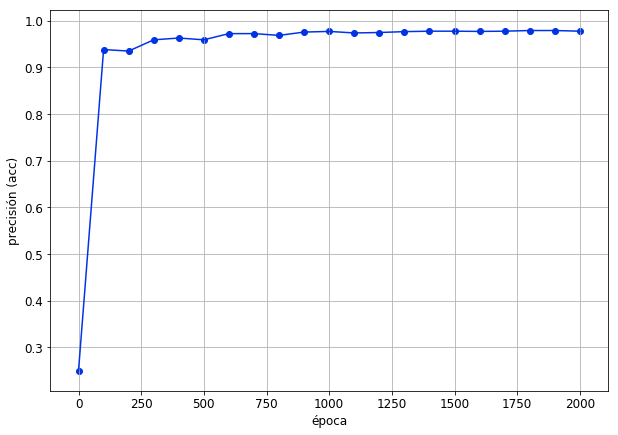
\includegraphics[scale=0.3]{model1}}
\qquad
\subfloat[2 Convo 2 FC]{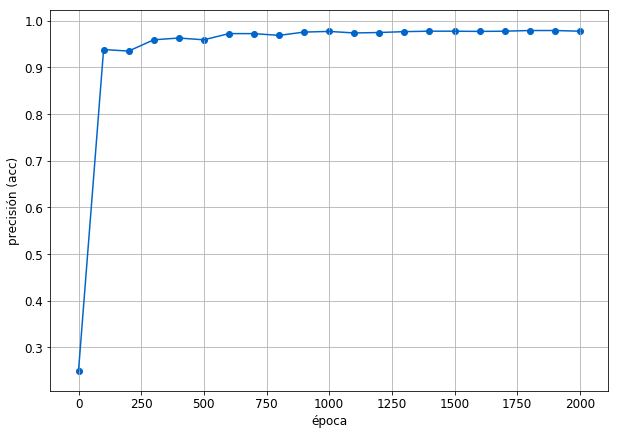
\includegraphics[scale=0.3]{model2}}
\qquad
\subfloat[2 Convo 1 FC]{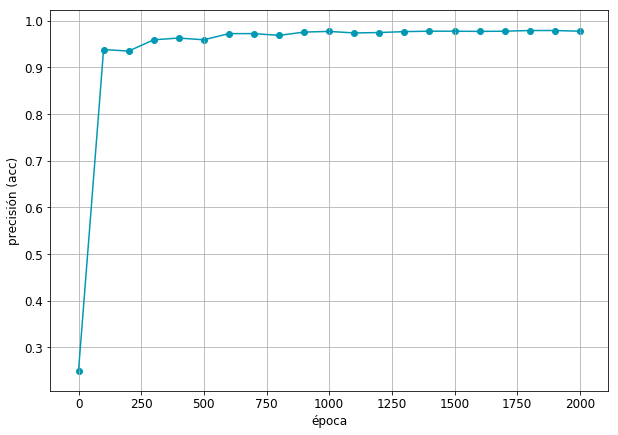
\includegraphics[scale=0.3]{model3}}
\qquad
\subfloat[1 Convo 2 FC]{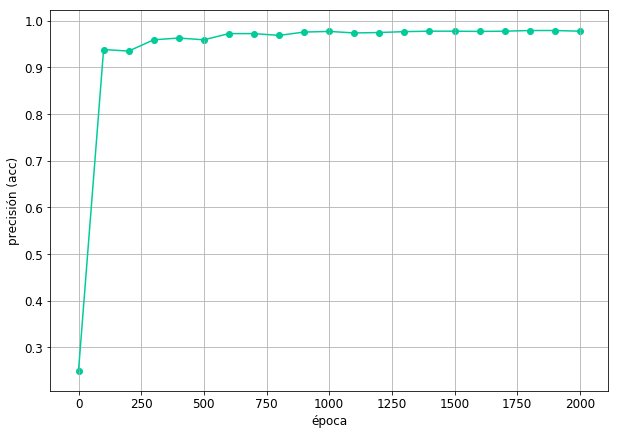
\includegraphics[scale=0.3]{model4}}
\qquad
\subfloat[1 Convo 1 FC]{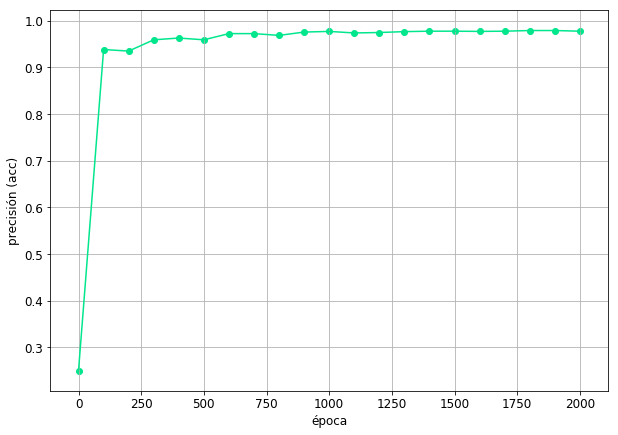
\includegraphics[scale=0.3]{model5}}
\caption{La precisión de cada modelo con respecto a las épocas.\label{fig:results_acc_epochs}}
\end{figure}


%
%\paragraph{Modelo 1}
%
%2 convo 2 FC
%
%\begin{table}[]
%\centering
%\caption{Modelo 1: 2 capas de convolución y una capa oculta}
%\label{table:red_one_2conv2fc}
%\begin{tabular}{|l|l|l|l|l|}
%\hline
%Época & Tiempo transcurrido & Error de entrenamiento & Error de prueba & Precisión    \\ \hline
%0     & 7.3202745914        & 3.0709540844           & 6.1779737473    & 0.2504734993 \\ \hline
%100   & 15.3162293434       & 0.246046558            & 0.2345223427    & 0.9384469986 \\ \hline
%200   & 23.2666277885       & 0.2221536636           & 0.1732220352    & 0.9351325631 \\ \hline
%300   & 31.2877190113       & 0.115122892            & 0.1277082711    & 0.9592803121 \\ \hline
%400   & 39.3300793171       & 0.0641306639           & 0.1061202958    & 0.9630681872 \\ \hline
%500   & 47.3877923489       & 0.0945049077           & 0.1096037999    & 0.9592803121 \\ \hline
%600   & 55.337015152        & 0.04487269             & 0.0840779245    & 0.9725378752 \\ \hline
%700   & 63.4053928852       & 0.0290345363           & 0.0777522177    & 0.9725378752 \\ \hline
%800   & 71.4111871719       & 0.0502839647           & 0.0865348205    & 0.96875      \\ \hline
%900   & 79.4459328651       & 0.0260504074           & 0.0731359869    & 0.9758522511 \\ \hline
%1000  & 87.4989733696       & 0.0170939807           & 0.0684150234    & 0.9772727489 \\ \hline
%1100  & 95.6583366394       & 0.0299351327           & 0.073277019     & 0.9739583135 \\ \hline
%1200  & 103.6676399708      & 0.0175534561           & 0.0689379498    & 0.9749053121 \\ \hline
%1300  & 111.7657170296      & 0.0112776877           & 0.0651408285    & 0.9767992496 \\ \hline
%1400  & 119.8008499146      & 0.0180956665           & 0.0692276433    & 0.9777461886 \\ \hline
%1500  & 127.9180393219      & 0.0126623595           & 0.06640324      & 0.9777461886 \\ \hline
%1600  & 135.9379198551      & 0.0079146475           & 0.0643871278    & 0.9772727489 \\ \hline
%1700  & 144.0074915886      & 0.0117598884           & 0.0699412525    & 0.9777461886 \\ \hline
%1800  & 152.1184546947      & 0.0093412921           & 0.0654446557    & 0.9791666865 \\ \hline
%1900  & 160.2102677822      & 0.0058462457           & 0.064642258     & 0.9791666865 \\ \hline
%2000  & 168.2911362648      & 0.0085604852           & 0.0712103397    & 0.9777461886 \\ \hline
%\end{tabular}
%\end{table}
%
%\paragraph{Modelo 2}
%
%2 convo 2 FC.
%
%
%\begin{table}[]
%\centering
%\caption{Modelo 2: 2 capas de convolución y una oculta}
%\label{table:2conv2fcbatch300}
%\begin{tabular}{|l|l|l|l|l|}
%\hline
%Época & Tiempo transcurrido & Error de entrenamiento & Error de prueba & Precisión    \\ \hline
%0     & 7.8421280384        & 2.8682234287           & 3.3460187912    & 0.241477266  \\ \hline
%100   & 16.9836273193       & 0.3026786149           & 0.2827074528    & 0.9214015007 \\ \hline
%200   & 26.0736353397       & 0.1818257272           & 0.1859790981    & 0.9441288114 \\ \hline
%300   & 35.2737841606       & 0.1262233555           & 0.1477904469    & 0.9498106241 \\ \hline
%400   & 44.4421823025       & 0.1001303717           & 0.1264027655    & 0.9550189376 \\ \hline
%500   & 53.6251189709       & 0.0818474591           & 0.1112083346    & 0.9554924369 \\ \hline
%600   & 62.7804038525       & 0.0689618215           & 0.1012903452    & 0.9625946879 \\ \hline
%700   & 72.0268294811       & 0.0598993674           & 0.0959407836    & 0.9659090638 \\ \hline
%800   & 81.1530988216       & 0.0549877919           & 0.0937793404    & 0.9659090638 \\ \hline
%900   & 90.3930594921       & 0.0481151342           & 0.0898199677    & 0.9696969986 \\ \hline
%1000  & 99.5937502384       & 0.0406286344           & 0.085127607     & 0.9734848738 \\ \hline
%1100  & 108.7840344906      & 0.0342642255           & 0.08182735      & 0.9749053121 \\ \hline
%1200  & 117.9713246822      & 0.0278111324           & 0.0783735365    & 0.9767992496 \\ \hline
%1300  & 127.1896910667      & 0.0229252577           & 0.0762095153    & 0.9772727489 \\ \hline
%1400  & 136.4318993092      & 0.0191811435           & 0.0749697983    & 0.9782196879 \\ \hline
%1500  & 145.6369526386      & 0.0163648594           & 0.0740553215    & 0.9786931872 \\ \hline
%1600  & 154.8179557323      & 0.0139603755           & 0.0733383074    & 0.9791666865 \\ \hline
%1700  & 164.0475275517      & 0.0120949261           & 0.0730332807    & 0.9786931872 \\ \hline
%1800  & 173.2340805531      & 0.0105913281           & 0.0729769841    & 0.9772727489 \\ \hline
%1900  & 182.4875264168      & 0.0094167981           & 0.0730196685    & 0.9772727489 \\ \hline
%2000  & 191.7189230919      & 0.0084654102           & 0.0732315555    & 0.9772727489 \\ \hline
%\end{tabular}
%\end{table}
%
%\paragraph{Modelo 3}
%
%2 covo 1 FC.
%
%\begin{table}[]
%\centering
%\caption{Modelo 3: 2 capas de convolución 1 completamente conectada}
%\label{table:model3}
%\begin{tabular}{|l|l|l|l|l|}
%\hline
%Época & Tiempo transcurrido & Error de entrenamiento & Error de prueba & Precisión    \\ \hline
%0     & 2.1028752327        & 5.429710865            & 7.2814497948    & 0.2642045319 \\ \hline
%100   & 6.0483319759        & 0.3088294864           & 0.3315916061    & 0.9057765007 \\ \hline
%200   & 9.9446578026        & 0.207638666            & 0.2255852371    & 0.9289772511 \\ \hline
%300   & 13.8171753883       & 0.3040256202           & 0.2913019061    & 0.9005681872 \\ \hline
%400   & 17.6553535461       & 0.1283937991           & 0.1651451886    & 0.9427083135 \\ \hline
%500   & 21.5917801857       & 0.1089217067           & 0.157908693     & 0.9403409362 \\ \hline
%600   & 25.4469769001       & 0.1987725496           & 0.1853734255    & 0.9346590638 \\ \hline
%700   & 29.3310687542       & 0.0858137906           & 0.1235252693    & 0.9602272511 \\ \hline
%800   & 33.225922823        & 0.0737339705           & 0.1292105466    & 0.9535984993 \\ \hline
%900   & 37.1445102692       & 0.1441168338           & 0.1384231746    & 0.9521780014 \\ \hline
%1000  & 41.0286338329       & 0.0607568994           & 0.1053966731    & 0.9692234993 \\ \hline
%1100  & 44.9228360653       & 0.0545381755           & 0.1131819487    & 0.9621211886 \\ \hline
%1200  & 48.7702672482       & 0.1076918915           & 0.1140853167    & 0.9616477489 \\ \hline
%1300  & 52.6551091671       & 0.0456284918           & 0.0980426818    & 0.9701704383 \\ \hline
%1400  & 56.4932639599       & 0.0431456864           & 0.1037823632    & 0.9673295617 \\ \hline
%1500  & 60.3736059666       & 0.0825673938           & 0.1017076969    & 0.9668560624 \\ \hline
%1600  & 64.2060873508       & 0.0358270295           & 0.0946439132    & 0.9701704383 \\ \hline
%1700  & 68.1200900078       & 0.034217272            & 0.0975136459    & 0.9706439376 \\ \hline
%1800  & 72.0071187019       & 0.0638250113           & 0.0943133309    & 0.9701704383 \\ \hline
%1900  & 75.883657217        & 0.0286074877           & 0.0940102115    & 0.9711174369 \\ \hline
%2000  & 79.7310190201       & 0.0272229407           & 0.0934648365    & 0.9715909362 \\ \hline
%\end{tabular}
%\end{table}
%
%
%
%\paragraph{Modelo 4}
%
%1 convo 2 FC.
%
%
%\begin{table}[]
%\centering
%\caption{Tabla 4: 2 capas de convolución 1 completamente conectada.}
%\label{table:model4}
%\begin{tabular}{|l|l|l|l|l|}
%\hline
%Época & Tiempo transcurrido & Error de entrenamiento & Error de prueba & Precisión    \\ \hline
%0     & 4.8190894127        & 3.4078867435           & 1.8335254192    & 0.2561553121 \\ \hline
%100   & 10.5430588722       & 0.2876966596           & 0.2554202676    & 0.9190340638 \\ \hline
%200   & 16.2716712952       & 0.2585280836           & 0.1728164405    & 0.9441288114 \\ \hline
%300   & 21.984313488        & 0.2033729404           & 0.1497282833    & 0.9446022511 \\ \hline
%400   & 27.6639053822       & 0.133350119            & 0.139832899     & 0.9464961886 \\ \hline
%500   & 33.3875226974       & 0.1221942604           & 0.1160472557    & 0.9635416865 \\ \hline
%600   & 39.071198225        & 0.1346343458           & 0.111930415     & 0.9663825631 \\ \hline
%700   & 44.7847318649       & 0.0859281719           & 0.1102579832    & 0.9592803121 \\ \hline
%800   & 50.4557569027       & 0.0763712376           & 0.0923053026    & 0.9715909362 \\ \hline
%900   & 56.1923205853       & 0.0939286873           & 0.0953650922    & 0.9706439376 \\ \hline
%1000  & 61.9322435856       & 0.0572218187           & 0.0942356661    & 0.9678030014 \\ \hline
%1100  & 67.6439433098       & 0.0517053083           & 0.0810680985    & 0.9763257504 \\ \hline
%1200  & 73.3566286564       & 0.0669792295           & 0.0883587152    & 0.9730113745 \\ \hline
%1300  & 79.0891780853       & 0.0388560072           & 0.0845807865    & 0.9734848738 \\ \hline
%1400  & 84.7962470055       & 0.0358598083           & 0.07602036      & 0.9772727489 \\ \hline
%1500  & 90.4903838634       & 0.0488497727           & 0.0864205137    & 0.9725378752 \\ \hline
%1600  & 96.1585409641       & 0.0279216766           & 0.0798797309    & 0.9763257504 \\ \hline
%1700  & 101.8997781277      & 0.0248262715           & 0.0739214197    & 0.9777461886 \\ \hline
%1800  & 107.6456582546      & 0.0374025591           & 0.0860014334    & 0.9734848738 \\ \hline
%1900  & 113.370872736       & 0.0207491834           & 0.0776060075    & 0.9772727489 \\ \hline
%2000  & 119.1330387592      & 0.0177799109           & 0.0743050575    & 0.9767992496 \\ \hline
%\end{tabular}
%\end{table}
%
%\paragraph{Modelo 5}
%
%1 convo 1 FC.
%
%\begin{table}[]
%\centering
%\caption{Modelo 5: 1 capa de convolución 1 capa completamente conectada}
%\label{table:model5}
%\begin{tabular}{|l|l|l|l|l|}
%\hline
%Época & Tiempo transcurrido & Error de entrenamiento & Error de prueba & Precisión    \\ \hline
%0     & 1.3093357086        & 1.9210841656           & 1.9909992218    & 0.2334280312 \\ \hline
%100   & 3.5064704418        & 0.4699867666           & 0.3694962263    & 0.9019886255 \\ \hline
%200   & 5.718821764         & 0.2064059079           & 0.2735858858    & 0.9195075631 \\ \hline
%300   & 7.9507069588        & 0.321207583            & 0.2440538406    & 0.9180871248 \\ \hline
%400   & 10.1652519703       & 0.2827648222           & 0.2159627676    & 0.9261363745 \\ \hline
%500   & 12.399163723        & 0.1229303852           & 0.200532645     & 0.9313446879 \\ \hline
%600   & 14.6175277233       & 0.2280674428           & 0.192340821     & 0.9299242496 \\ \hline
%700   & 16.8630867004       & 0.2157354206           & 0.1778713614    & 0.9308711886 \\ \hline
%800   & 19.0751066208       & 0.0978225544           & 0.1696051657    & 0.9384469986 \\ \hline
%900   & 21.3231885433       & 0.1785159856           & 0.1666600704    & 0.9370265007 \\ \hline
%1000  & 23.5529901981       & 0.1691013724           & 0.1553606391    & 0.9427083135 \\ \hline
%1100  & 25.7864727974       & 0.0828434825           & 0.1507069916    & 0.9441288114 \\ \hline
%1200  & 28.0087628365       & 0.1457120925           & 0.1495355666    & 0.9450757504 \\ \hline
%1300  & 30.241517067        & 0.1372746676           & 0.1403872371    & 0.9493371248 \\ \hline
%1400  & 32.4557955265       & 0.0717598572           & 0.1377647668    & 0.9535984993 \\ \hline
%1500  & 34.7012207508       & 0.1211939454           & 0.1370747089    & 0.9507575631 \\ \hline
%1600  & 36.9285581112       & 0.1132190526           & 0.1292845905    & 0.9554924369 \\ \hline
%1700  & 39.1642153263       & 0.0621341504           & 0.1280657798    & 0.9569128752 \\ \hline
%1800  & 41.3848059177       & 0.1034243405           & 0.1276608855    & 0.9550189376 \\ \hline
%1900  & 43.6157948971       & 0.0946448147           & 0.120853819     & 0.9592803121 \\ \hline
%2000  & 45.837754488        & 0.055428572            & 0.1209859028    & 0.9611742496 \\ \hline
%\end{tabular}
%\end{table}
%
%%Los modelos con la mayor precisión sobre todos son el modelo uno y
%%dos con una proporción de valores correctamente clasficados del
%%0.9791666865. Se puede ver que los parámetros que comparten todas
%%las arquitecturas son el número de épocas y la tasa de aprendizaje,
%%además de que en sus kernels aparece al menos uno con una dimensión 
%%de $5 \times 5$.
%
%%
%%\end{document}


\subsubsection{Pruebas sobre el robot NAO}

Para finalizar la implementación del modelo sobre la arquitectura
se debe integrar uno de los cinco modelos descritos en la tabla \ref{table:models_results} sobre la API REST de CloudNAO y luego hacer peticiones con el robot a ésta.
Los modelos elaborados en TensorFlow contienen la gráfica de cómputo
y los valores de los parámetros que se han entrenado. Estos datos
están contenidos en varios archivos que se pueden guardar para
entrenamientos posteriores o para realizar inferencias sobre 
un modelo cuyas variables han sido aprendidas.

Se eligió el modelo con la precisión más alta y con el menor
tiempo de entrenamiento que es el modelo (1). 
%Durante la ejecución
%de la gráfica del modelo se crea una instancia de la clase \texttt{tf.train.Saver()}. Esto crea cuatro archivos
%uno con extensión \texttt{.meta}, uno con extensión \texttt{.index},
%otro con extensión \texttt{.data} y otro sin extensión llamado
%\texttt{checkpoint}. El primero guarda toda la gráfica de
%TensorFlow, los otros tres almacenan los valores de las variables.
%Después de guardar, simplemente se restaura el modelo
%y se puedan hacer inferencias al alimentarlo con una imagen.
Dentro de la API REST, la clase que se encarga de restaurar la gráfica y valores del modelo
es \texttt{ImageClasssfier} dentro del módulo \texttt{indoor\_scenes\_classsifier} del paquete \texttt{tf\_models}.
En el apartado \textit{Modelos de TensorFlow (tf\_models)}
de la sección \ref{chapter_two/desc_cloudnao:api-rest-de-cloudnao}
se describe cómo utilizar esta clase.

Por otra parte el robot NAO o cualquier otro
dispositivo cliente se comunica con la API a través
de una biblioteca que permita hacer peticiones 
HTTP. En el caso del robot ocupamos la biblioteca
\texttt{requests} de Python. Para obtener una imagen 
del robot codificada en base 64 se utilizó la clase \texttt{Robot}
del módulo \texttt{nao\_robot} descrito en la sección
\ref{\detokenize{firebase-nao-robot}}. Es la cadena
que representa la imagen la que se envía a la API REST usando
\texttt{requests}.

En la figura \ref{nao_api_images} se muestran algunas imágenes 
de $160 \times 120$ pixeles y las
respuestas enviadas por el servicio de clasificación
de escenarios dentro del recurso \texttt{vision} de la
API REST de CloudNAO.


\begin{figure}[!ht] 
  \centering
  
\subfloat[Clase = zona de trabajo, predicción = zona de trabajo. Tiempo = 3.02]{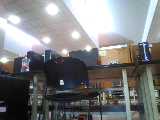
\includegraphics[scale=1]{nao_api_desk}}
\qquad
\subfloat[Clase = salida, predicción = salida. Tiempo = 3.12]{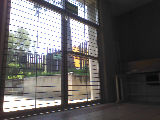
\includegraphics[scale=1]{nao_api_exit}}
\qquad
\subfloat[Clase = oficina, predicción = salida. Tiempo = 2.78]{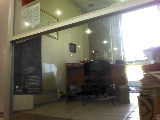
\includegraphics[scale=1]{nao_api_office}}
\qquad
\subfloat[Clase = cancha, predicción = cancha. Tiempo = 3.57]{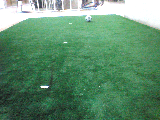
\includegraphics[scale=1]{nao_api_soccer}}
\caption{Predicciones hechas enviando imágenes del robot a la API REST. El tiempo son los
segundos que se tardó en enviar la solicitud y en recibir la respuesa. \label{nao_api_images}}
\end{figure}







 

